% !TEX encoding = UTF-8 Unicode
% !TEX root = ../thesis.tex


\begin{figure}[t]    
\centering
	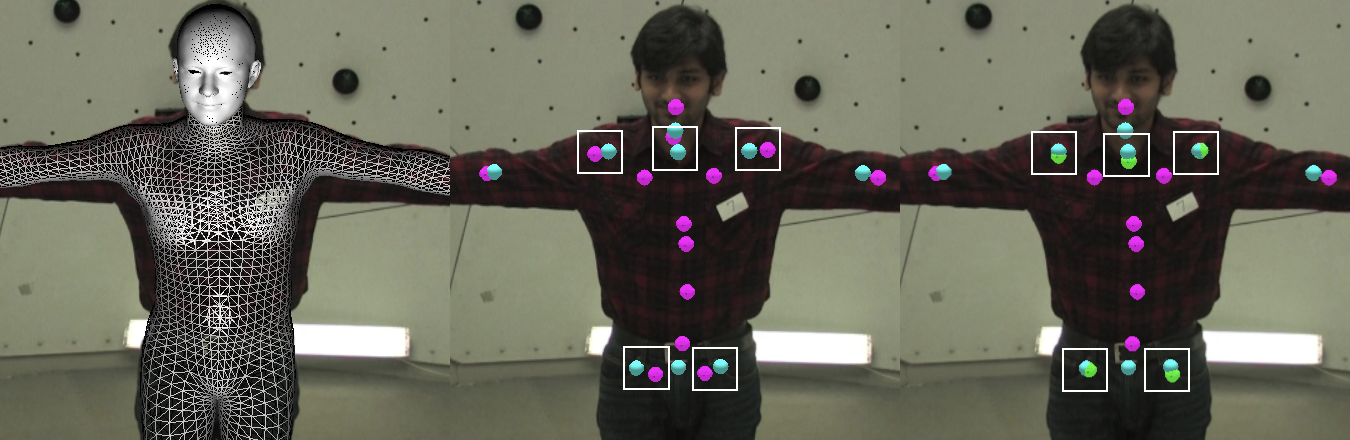
\includegraphics[width=\columnwidth]{tbc_figures/Jointregression_detectionTarget_nospace}    
	%\includegraphics[width=0.9\columnwidth]{fig/detectionTarget_legend}   
	\caption{Regressing detection target 3D positions. (Left) The template model is aligned with target object; (Mid.) The torso joints of the template model (magenta) have discrepancy from the joint definitions of 3D keypoint detection (cyan); (Right) The newly regressed target locations (green) are more consistent with 3D keypoint detections.}
	\label{fig:jointRegression}
\end{figure}
%
%
%\begin{figure}[t]    
%	\includegraphics[width=\columnwidth]{fig/Jointregression_coloradjus}  
%	\label{fig:adam_jointRegression}
%	\caption{We train a new regression function to compute joints from mesh vertices based on the reconstructed hundreds people's examples. (a) Projected mesh on an example image showing that the template model is aligned with target object. (b) The torso joints of the template model (magenta) have discrepancy from the joint definition of 3D detection measurements (cyan). (c) Newly regressed joints of our method are shown as green (d) Our joints definition (green)is more consistent to the joints from detection (cyan). }
%\end{figure}	

%\section{Building Total Model}
\section{Creating Adam}
We derive a new model, Adam, enabling total body motion capture with a simpler parameterization than the part-based Frank model. In particular, this new model has a single joint hierarchy and a common parameterization for all shape degrees of freedom, tying together the face, hand, and body shapes and avoiding the need for separate part parameterizations or seam constraints. To build the model, it is necessary to align the reconstructed meshes with all body parts (face, body, and hands) of diverse subjects where the model can learn the variations. To do this, we leverage our Frank model and apply it on a dataset of 70 subjects where each of them performs a short range of motion in a multiview camera system. We select 5 frames for each person in different poses, resulting in 350 meshes, and reconstruct them with our Frank model, producing aligned meshes with joint locations to build Adam. Because we derive the model from clothed people, the blendshapes explain variations of clothing at a coarse level.% due to the bulk of clothes and hair.

%while wearing everyday clothing. During the capture, we asked them to perform a T-pose and an action of their choosing. We selected 5 frames for each person with different poses and fit the Frankenstein model to each frame independently, which are then used to build Adam. Because we derive the model from clothed people, the linear shape blendshapes explain some variation in geometry due to the bulk of clothes and hair, which leads to better surface matching during ICP.
%We build a new model, named the TOTAL MODEL, to capture to solve the issued arising in the Frankenstein model. To achieve this, we collect a large scale humna dataset with natural hairs, clothing, and motions. We use the Frankenstein Model to compute the motion and shape for the people, and also reconstruct the out-of-model shapes by computing normal-direction delta shape parameters. To this end, we build a new linear blend shapes to cover the clothing and hairs. We also additional tuned the joint location to be consistent with detection cost. The final optimization framework is much simpler and more generally usable than the Frankenstein models. 
%We collect a short range of motion sequence from 70 people,  Examples are shown in Fig.~\ref{fig:compare_franken_adam}.


%\subsection{Reconstructing out-of-model space}
\subsection{Fitting Clothes and Hair}
%The output of the previous fitting still contains shapes in the model space. 
The Frank model captures the shape variability of human bodies and faces, but does not account for clothing or hair, since it keeps the original model space of part models (\cite{Loper2015} and \cite{cao2014facewarehouse}). To learn a new set of linear blendshapes that better capture the rough geometry of clothed people and also roughly model hair, we need the meshes to match the geometry of the source data more accurately. For this purpose, we deform the meshes outside of the shape-space along each the normal direction of each vertex. For each vertex $\mathbf{v}_i $ in the Frank model, the deformed mesh vertex $\tilde{\mathbf{v}}_i$ is represented as:
\begin{align}
\tilde{\mathbf{v}}_i  =  \mathbf{v}_i  + \mathbf{n}(\mathbf{v}_i) \delta_i,
\end{align}
where $\delta_i \in \mathds{R} $ is a scalar displacement meant to compensate for the discrepancy between the Frank model vertices and the 3D point cloud, along the normal direction at each vertex. 
% However, directly computing this from closest-point correspondences can produce severe artifacts, as the 3D point clouds are noisy and contain large holes due to failed stereo matching. We therefore use a Laplacian shape prior\cite{} to regularize the deformations and introduce visibility and normal matching constraints to reject incorrect correspondences. 
%Finally, we run the optimization over multiple frames together with a shared $\Delta$ parameters
%\textbf{Laplacian Shape constraints}
We pose the problem as a linear system,
% transform the current vertex $\mathbb{V}$ to be close to the target point cloud set $\mathbf{P}$, with Laplacian of the mesh is maintained:
%\begin{align}
%\mathbf{V} +N\cdot\Delta = \mathbf{P}\\
%L\cdot \left( \mathbf{V} + N\cdot\Delta \right) - L\cdot\mathbf{V} = 0
%%L\cdot \left( N\cdot\Delta \right) = 0
%\end{align}
%Since all terms are linear, we can concatenate them to build a linear system:
%
\begin{align}
\label{eq:delta_recon}
\begin{pmatrix} \mathbf{N}^T  \\ (\mathbf{W} \mathbf{L} \mathbf{N})^T  \end{pmatrix} \Delta
= \begin{pmatrix} (\mathbf{P} - \mathbf{V}^U)^T \\ \mathbf{0} \end{pmatrix},
\end{align}
where $\Delta\in\mathds{R}^{N^U}$ contains the stacked per-vertex displacements, $\mathbf{V}^U$ are the vertices in the Frank model, $\mathbf{P}\in\mathds{R}^{N^U\times 3}$ are corresponding point cloud points, $\mathbf{N}\in\mathds{R}^{N^U\times 3}$ contains the mesh vertex normals, and $\mathbf{L}\in\mathds{R}^{N^U\times N^U}$ is the Laplace-Beltrami operator to regularize the deformation. We also use a diagonal weight matrix $\mathbf{W}\in\mathds{R}^{N^U\times N^U}$ to avoid large deformations where the 3D point cloud has lower resolution than the original mesh, such as details in the face and hands. %After reconstructing $\Delta$, the generated output models shows better 
% \textbf{Visibility Maps: } 
% Deforming out of model space can introduce artifacts if false correspondences are established with the noisy point clouds that we get from our limited resolution cameras. 
% % This is particularly true with the point cloud reconstructions we were able to get with the limited resolution of our multicamera system. 
% Problematic regions include joint regions, where association can match points to a different body part. To avoid this, we discard ``unreliable'' correspondences using a visibility heuristic. We compute the visibility of every vertex from the cameras used to reconstruct the point cloud, and use this as a reliability measure: if a vertex is not visible from sufficient cameras, it is unlikely to have a corresponding 3D match, so we do not correspond such difficult areas (e.g., below the arms, between the legs). 

% \textbf{Multi Frame Fitting: } To further reduce noise, we solve for the surface $\Delta$ using multiple frames simultaneously. This can be done by stacking the linear constraints in Eq.~\ref{eq:delta_recon} obtained from multiple frames in a single system. 
%\begin{align}
%\begin{pmatrix} \mathbf{N}_1  \\ \mathbf{L}\cdot \mathbf{N}_2 \\ \mathbf{N}_2  \\ \mathbf{L}\cdot \mathbf{N}_1 \\ \cdots \end{pmatrix} \Delta
%= \begin{pmatrix} \mathbf{P}_1 - \mathbf{V}_1 \\ \mathbf{0}  \\ \mathbf{P}_2 - \mathbf{V}_2 \\ \mathbf{0} \\ \cdots \end{pmatrix}
%\end{align}

%\begin{figure}[t]	
%	\includegraphics[width=0.32\columnwidth,trim=800 80 500 90, clip]{fig/visibility_corres/visibility_5frames_1iter}
%	\includegraphics[width=0.32\columnwidth,trim=800 80 500 90, clip]{fig/visibility_corres/1_1iter_noVis}	
%	\includegraphics[width=0.32\columnwidth,trim=800 80 500 90, clip]{fig/visibility_corres/1_1iter_visibility_1frames}
%	%\includegraphics[width=0.24\columnwidth,trim=0 0 0 0, clip]{fig/visibility_corres/visibilityMap}	
%	
%	\caption{Delta Reconstruction Results. (a) Original Frankenstein model output; (b) Delta deformation without visibility map; (c) Delta deformation with visibility map; (D) color coded visibility map (blue with low visibility, and red with high visibility).}
%	\label{fig:deltarecon}
%\end{figure}
%

% \begin{figure}[t]    
% 	\includegraphics[width=\columnwidth]{fig/compare_franken_adam}    
% 	%\includegraphics[width=\columnwidth]{fig/compare_franken_adam2}    
% 	\caption{Comparison between the shape space of Frankenstein model and Adam model. For each example, (left) an input image; (middle) Frankenstein model fitting result; (right) Adam model fitting result with the same 3D measurements.}
% 	\label{fig:compare_franken_adam}
% \end{figure}

% Emphasize this section in the contribution. 
% There's a disconnect between the joints and the output of the detectors. Detector target regressor?

%\subsection{Regressing New Joint Locations}
\subsection{Detection Target Regression}
There exists an important discrepancy between the joint locations of the LBS model (i.e., the 3D centers of rotation for bone deformation) and the location of the keypoint detections (which come from manually annotated guesses of where the anatomical joints are in 2D images). This is shown in Fig.~\ref{fig:jointRegression}. This difference has the effect of pulling the model towards a bad fit even while achieving a low keypoint cost, $E_{\textrm{keypoints}}$, especially for shoulders and hips. We alleviate this problem by computing a new regression function, $\mathbf{\hat{J}}^A \in \mathds{R}^{J^A\times N^U}$, which relates the vertices in the body model to the expected location of 3D keypoint detections. However, to be able to learn these regressors, we require instances of the fitted model vertices as well as the 3D keypoint detections.


Therefore, we first fit the Frank model (with additional shape variations) using the original joint locations as detection targets, and obtain aligned meshes across all subjects. Based on these outputs, we can build the regression matrix using the  locations of 3D keypoint measurements as targets instead of Frank model's joint locations. Similar to the joint regression in SMPL~\cite{Loper2015}, we first select a subset of vertices in the proximity of each detection target, and estimate a fixed, sparse linear combination of these vertices that approximates the location of the 3D keypoint across all fitted meshes. This optimization is posed as an L1-regularized least-squares problem with non-negative constraints, where we additionally impose that the vertex weights sum to one, resulting in an interpolation. 

The results are shown in Fig.~\ref{fig:jointRegression}. Note that this new regressor is used only for the optimization in Eq.~\eqref{eq:detection_eq}, whereas the original joint regressor from SMPL~\cite{Loper2015}, $\mathbf{J}^A$, is used for LBS. However, we also add rows to the joint regression matrix to account for the additional finger joints, which we solve for in the same way. The resulting matrix is $\mathbf{J}^A \in \mathds{R}^{J^A\times N^U}$ where $N^U$ is the number of vertices of Adam (the same as Frank) and $J^A=61$ is the number of joints in Adam model including 21 body joints and 20 finger joints (including 5 finger tips) for each hand. 

 %a 3D detection, and then estimate a fixed, sparse linear combination of these vertices that approximates the location of the 3D keypoint across all fitted meshes. This is posed as as L1-regularized least squares problem with non-negative constraints, where we additionally impose that the vertex weights sum to one, resulting in an interpolation. We found that we achieved best results by solving this problem iteratively, starting from a large set of candidate vertices and then removing vertices with zero or low weights, and then repeating the procedure with the new candidate set until each detection uses fewer than 10 vertices as interpolators. These new regression weights are then used to generate correspondences to the detection targets in $E_\textrm{keypoints}$. 


%The problem can be alleviated by also fitting the mesh surface to the MVS point clouds using ICP. This leads to a better overall fit, but a higher $E_{\textrm{keypoints}}$ cost, as the SMPL joints and the 3D detections will no longer be perfectly aligned. 



%the relative location of the 3D detections with respect to the fitted mesh vertices by leveraging the the reconstructed 70 people data. This allows us to define new targets for the keypoint detection cost that, on average, are a better match for the location of the 3D detections with respect to the mesh model, as shown in Fig.~\ref{fig:jointRegression}. In particular, given the fitting results of 70 identities, we approximate the target 3D keypoint locations as a function of the final fitted mesh vertices following the procedure of~\cite{Loper2015} to find a sparse, linear combination of vertices that approximates the position of the target 3D keypoint. Note that we do not change the joint location used in the skeleton hierarchy during LBS deformation, only the regression matrices $\mathbf{J}_i$ in Eq.~\eqref{eq:detection_eq}. %This can be also applied on Farnkenstein model. 
%Original
%There exists a discrepancy between the SMPL body joint locations and the location of the keypoint detections used in the OpenPose body detector (i.e., a model joint vs. a detection joint). This affects mainly the shoulder and hip joints, which are not only difficult to annotate on clothed people, but are also difficult to model accurately in an LBS framework, which results in non-anatomical placements for these joints. This difference in their definition has the effect of pulling the Frankenstein model towards a bad fit even while achieving a low keypoint cost, $E_{\textrm{keypoints}}$. The problem can be alleviated by also fitting the mesh surface to the MVS point clouds using ICP. This leads to a better overall fit, but a higher $E_{\textrm{keypoints}}$ cost, as the SMPL joints and the 3D detections will no longer be perfectly aligned. We alleviate this problem by computing the relative location of the 3D detections with respect to the fitted mesh vertices by leveraging the the reconstructed 70 people data. This allows us to define new targets for the keypoint detection cost that, on average, are a better match for the location of the 3D detections with respect to the mesh model, as shown in Fig.~\ref{fig:jointRegression}. In particular, given the fitting results of 70 identities, we approximate the target 3D keypoint locations as a function of the final fitted mesh vertices following the procedure of~\cite{Loper2015} to find a sparse, linear combination of vertices that approximates the position of the target 3D keypoint.
% We follow a similar procedure as used in \cite{Loper2015} to define the location of SMPL joints as a function of mesh vertices. 
% We first select a subset of vertices in the proximity of a 3D detection, and then estimate a fixed, sparse linear combination of these vertices that approximates the location of the 3D keypoint across all fitted meshes. This is posed as as L1-regularized least squares problem with non-negative constraints, where we additionally impose that the vertex weights sum to one, resulting in an interpolation. We found that we achieved best results by solving this problem iteratively, starting from a large set of candidate vertices and then removing vertices with zero or low weights, and then repeating the procedure with the new candidate set until each detection uses fewer than 10 vertices as interpolators. These new regression weights are then used to generate correspondences to the detection targets in $E_\textrm{keypoints}$. 
%Note that we do not change the joint location used in the skeleton hierarchy during LBS deformation, only the regression matrices $\mathbf{J}_i$ in Eq.~\eqref{eq:detection_eq}. 

\subsection{Building the Shape Deformation Space}

After model fitting with $\Delta$ displacement, we warp each frame's surface to the rest pose, applying the inverse of the LBS transform. With the fitted surfaces warped to this canonical pose, we do PCA analysis to build a joint linear shape space that captures shape variations across the entire body. As in Section~\ref{subsection:face}, we separate the expression basis for the face and retain the expression basis from the FaceWarehouse model, as our MVS point clouds are of too low resolution to fit facial expressions.
%To do that, we first export all the meshed in the rest poses, where all the pose parameters are zeros. Then, we run the similar method as we used to build the linear space for face, in subsection \ref{subsection:face}.

%The mean pose and example linear subspaces are shown in Fig.\ref{fig:totallinearspace}. 
%The a model now can have shape variation for all parts, including body, hand, and face. The model also includes deformation of hair and clothing. That is this model can substitute parameters of $\phi^F$, $\phi^B$, and $\phi^H$. 
The Adam model is parameterized as:
\begin{align}
M^A (\boldsymbol{\theta}^A, \boldsymbol{\phi}^A, \boldsymbol{t}^A ) = \mathbf{V}^A
\end{align}
with $\mathbf{V}^A = \{ \mathbf{v}^A_i\}_{i=1}^{N^A}$ and $N^A{=}18540$ which is equal to the vertices in Frank, $N^U$. As in SMPL, the vertices of this template mesh are first displaced by a set of blendshapes in the rest pose, $\hat{\mathbf{v}}^A_i = \mathbf{v}^{A0}_i + \sum_{k=1}^{K_A} \mathbf{s}^k_{i} \phi^A_k,$ 
where $\mathbf{s}^k_{i}\in\mathds{R}^3$ is the $i$-th vertex of the $k$-th blendshape, $\phi^A_k$ is the $k$-th shape coefficients of $\boldsymbol{\phi}^A\in\mathds{R}^{K_b}$, and $K_A=40$ is the number of identity coefficients, $\mathbf{v}^{A0}$ is the mean shape and $\mathbf{v}^{A0}_i$ is its $i$-th vertex. Note that these blendshapes now capture variation across the face, hands, and body. These are then posed using LBS as in Eq.~\eqref{eq:full_lbs_pose} after obtaining joint locations by the joint regressor matrix $\mathbf{J}^A$. %We define the joints and weights for LBS followoing the part models, which is further explained in the supplementary material. %of jointFor the joint regressor from mesh vertices %The joint locations for the LBS function are generated by a newly computed joint regressor from mesh vertices including finger joints, which are computed as a similar way of ~\cite{Loper2015}. We mainly rely on the joint definition and LBS weights from part models with the reconstructed range of motion dataset.


% \begin{align}
% \hat{\mathbf{v}}^T_i = \mathbf{v}^{T0}_i + \sum_{k=1}^{K_T} \mathbf{s}^k_{i} \phi^B_k,
% \label{eq:total_shape_coeffs}
% \end{align}
%
%\begin{figure}[t]	
%	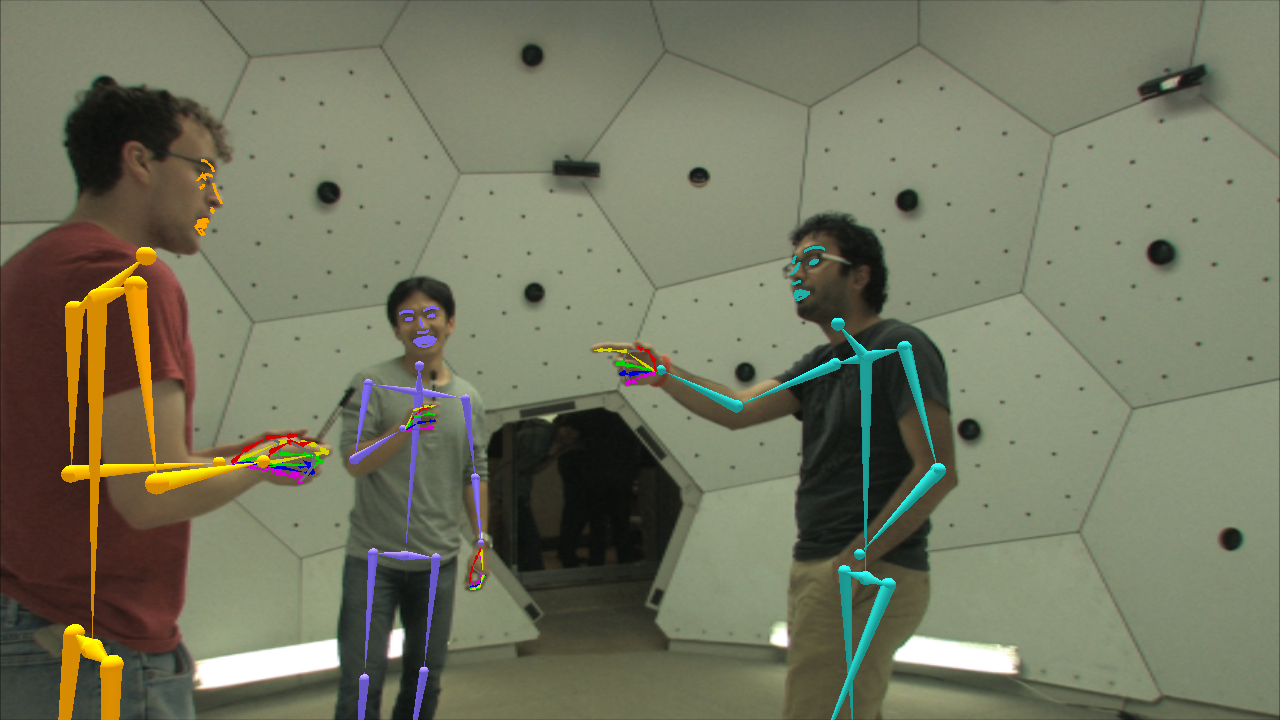
\includegraphics[width=0.24\columnwidth,trim=1000 110 1000 90, clip]{fig/totallinear/00000}
%	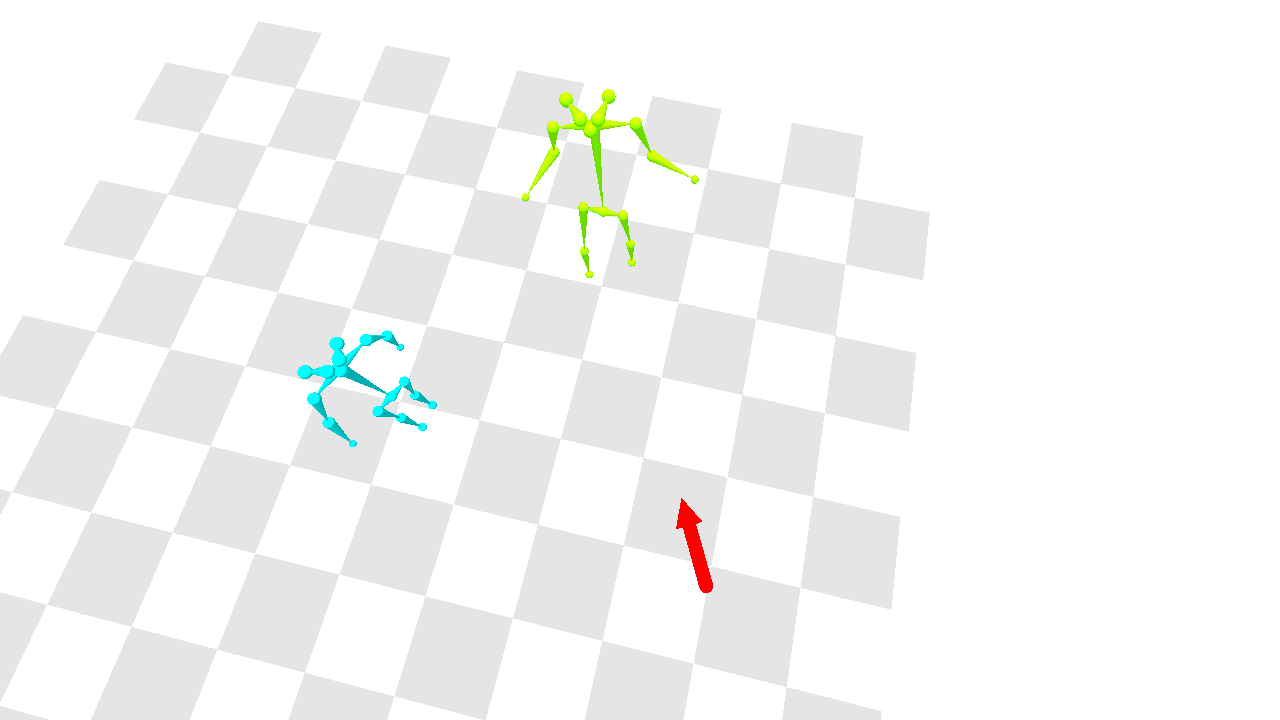
\includegraphics[width=0.24\columnwidth,trim=1000 110 1000 90, clip]{fig/totallinear/00001}	
%	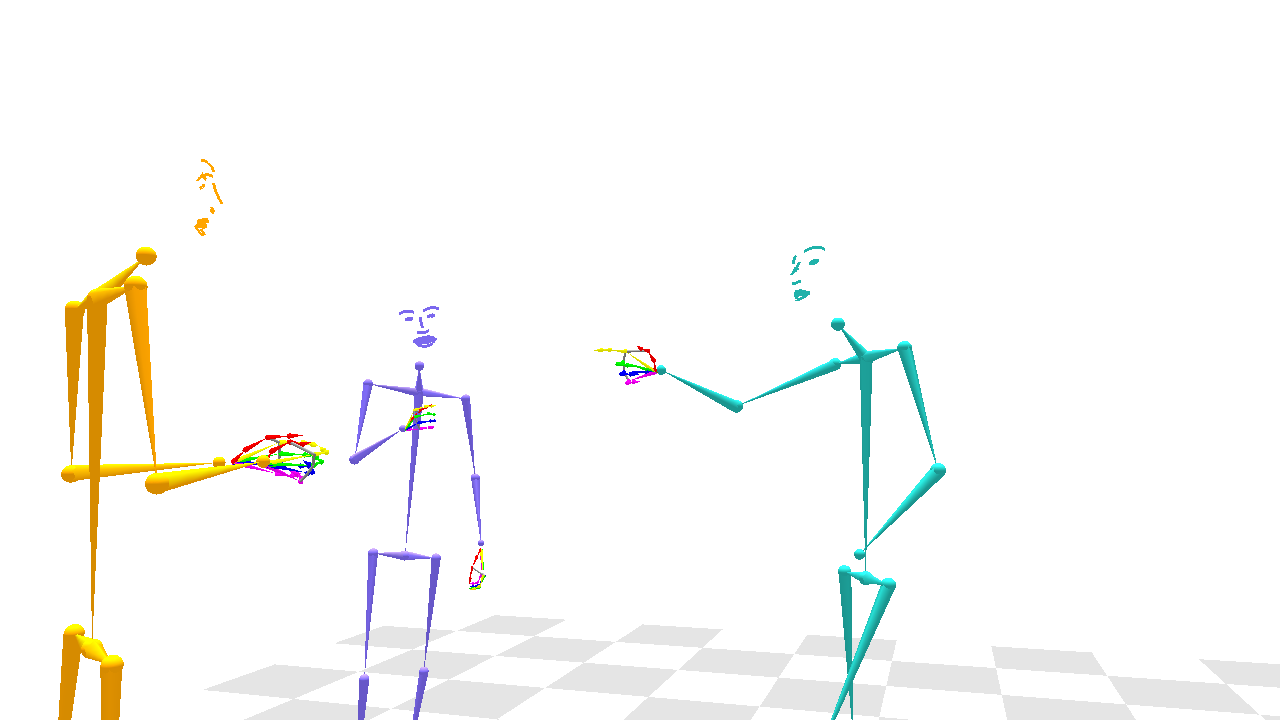
\includegraphics[width=0.24\columnwidth,trim=1000 110 1000 90, clip]{fig/totallinear/00002}
%	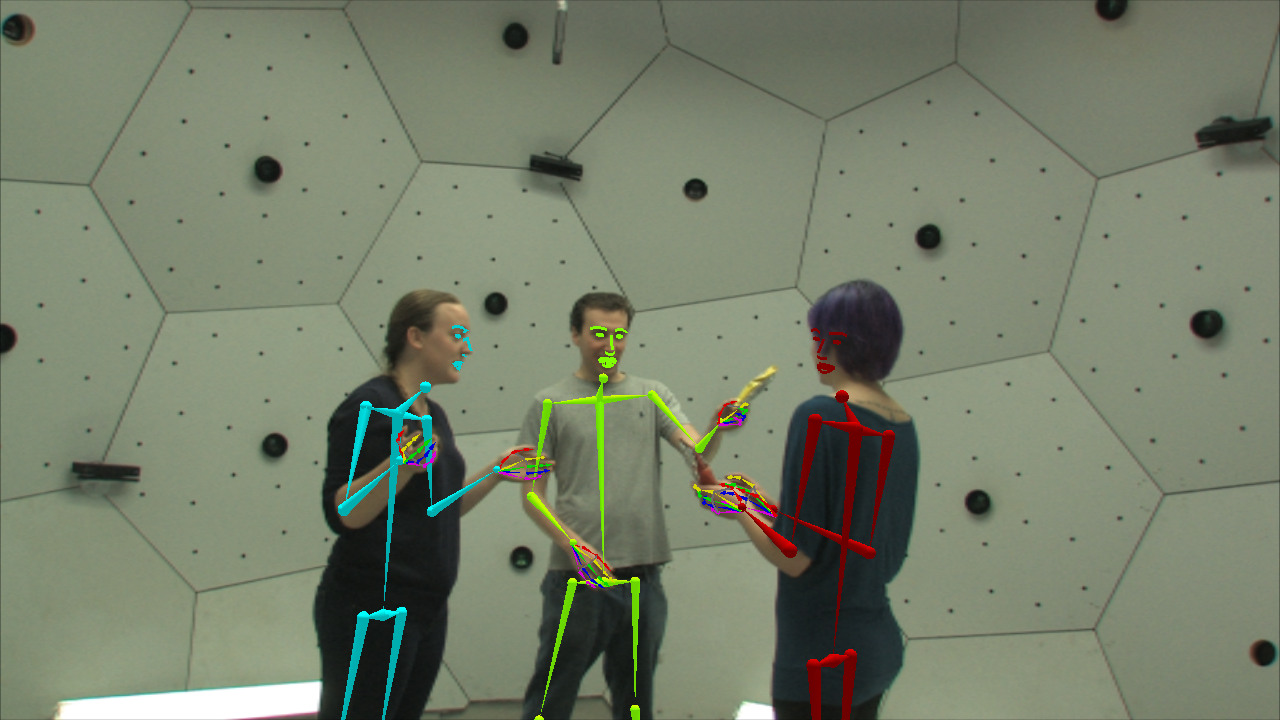
\includegraphics[width=0.24\columnwidth,trim=1000 110 1000 90, clip]{fig/totallinear/00003}	
%	\caption{Linear Blend Shapes for Total model. (a) mean shape; (b,c,d) after changing X-th,X-th,and X-th component respectively}
%	\label{fig:totallinearspace}
%\end{figure}
	
\subsection{Tracking with Adam}
% This section needs to be beefed up.
% Informal
The cost function to capture total body motion using Adam is similar to Eqn.~\ref{eq:fitting_franken} without the seam term:% ($E_\textrm{seam}$): 
\begin{align}
\label{eq:fitting_adam}
E\big( \boldsymbol{\theta}^A, \boldsymbol{\phi}^A, \boldsymbol{t}^A\big) = E_\textrm{keypoints} + E_\textrm{icp} +E_\textrm{prior}.
\end{align}
However, Adam is much more amenable to optimization than Frank: it has a single set of unified shape and pose parameters for all parts, and does not require seam constraints between disparate models. 
% Too informal

% The biggest advantage is setting the ratio among terms. E.g., seam term is tricky compared to others. 


%Conceptually, it is based on the SMPL model parameterization~\cite{Loper2015}, but with additional joints for the hands and facial expression blendshapes.

%\textbf{Optical Flow Propagation}: While fitting each frame independently has benefits----it does not suffer from error accumulation and frames can be fit in parallel---it typically produces jittery motion. To reduce this jitter, we use optical flow to propagate the initial, per-frame fit to neighboring frames to find a smoother solution. More concretely, given the fitting results at the frame $t$, we propagate this mesh to  frames $t{-}1$ and $t{+}1$ using optical flow at each vertex, which is triangulated into 3D using the method of~\cite{Joo2014}. Therefore, each vertex has at most three candidate positions: the original mesh, and the forward and backward propagated vertices (subject to a forward-backward consistency check). Given these propagated meshes, we reoptimize the model parameters by using all propagated mesh vertices as additional keypoints to find a compromise mesh. 
% In this case, every vertex has corresponding target locations by the propagated meshes. 
%We run this process multiple times (3, in our case), to further reduce jitter and fill in frames with missing detections.


